%%%%%%%%%%%%%%%% Relojes Bloom.
\begin{frame}[fragile]{Relojes Bloom:}{Algoritmo.}
  \justifying
  A continuación se describe el algoritmo usado en la
  dispersión de tiempos:
  \begin{enumerate}
  \item Definimos el tamaño del \textit{bloom-filtro-conteo}
    $m$ y las $k$ \textit{hash-funciones}.
  \item Cada vez que un nodo tiene un evento interno, procesa ese evento
    con $k$ \textit{hash-funciones} e incrementa su filtro. Luego envía
    ese filtro de floración a todos los demás nodos.
  \item Cada vez que un nodo recibe un evento, actualiza su filtro
    tomando el valor máximo de su filtro y el filtro receptor.
  \end{enumerate}
  \textbf{Ejemplo:}
      \begin{figure}
    \centering
    \begin{subfigure}[b]{0.45\textwidth}
      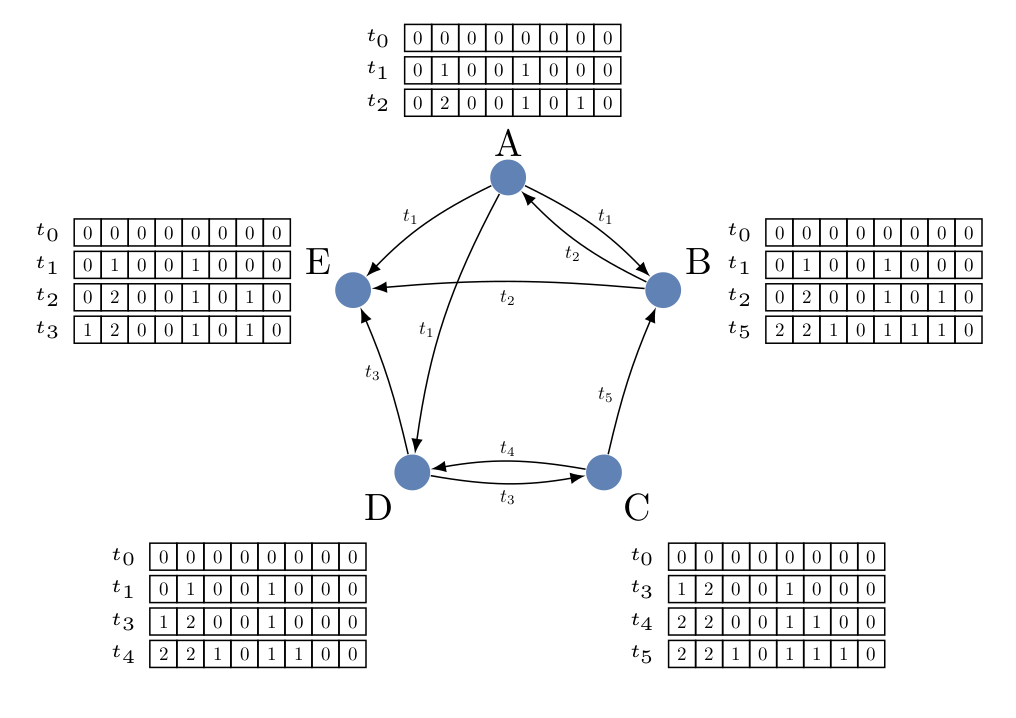
\includegraphics[width=\textwidth]{./Imagenes/RelojBloom}
      \caption{Reloj de Bloom.}
      \label{fig:Ejemplo de un CountingBloomClock.}
    \end{subfigure}
  \end{figure}
\end{frame}

\begin{frame}[fragile]{Relojes Bloom:}{Ejecución.}
  \justifying
  \textbf{Ejemplo:}
      \begin{figure}
    \centering
    \begin{subfigure}[b]{0.8\textwidth}
      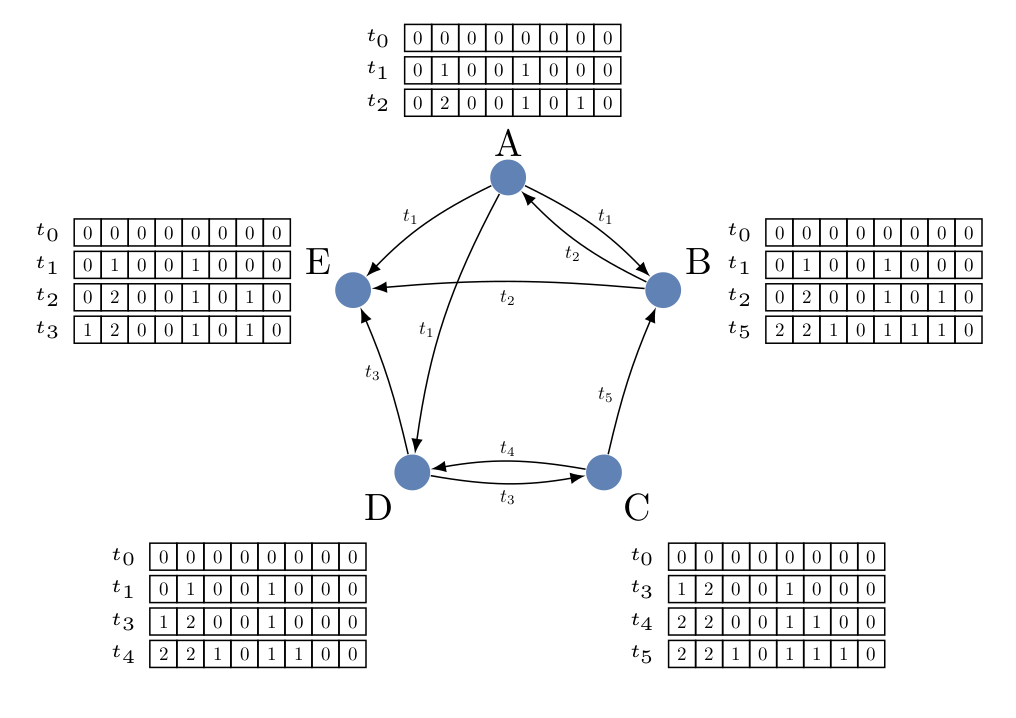
\includegraphics[width=\textwidth]{./Imagenes/RelojBloom}
      \caption{Reloj de Bloom.}
      \label{fig:Ejemplo de un CountingBloomClock.}
    \end{subfigure}
  \end{figure}
\end{frame}
